% Options for packages loaded elsewhere
\PassOptionsToPackage{unicode}{hyperref}
\PassOptionsToPackage{hyphens}{url}
%
\documentclass[
]{article}
\usepackage{amsmath,amssymb}
\usepackage{iftex}
\ifPDFTeX
  \usepackage[T1]{fontenc}
  \usepackage[utf8]{inputenc}
  \usepackage{textcomp} % provide euro and other symbols
\else % if luatex or xetex
  \usepackage{unicode-math} % this also loads fontspec
  \defaultfontfeatures{Scale=MatchLowercase}
  \defaultfontfeatures[\rmfamily]{Ligatures=TeX,Scale=1}
\fi
\usepackage{lmodern}
\ifPDFTeX\else
  % xetex/luatex font selection
\fi
% Use upquote if available, for straight quotes in verbatim environments
\IfFileExists{upquote.sty}{\usepackage{upquote}}{}
\IfFileExists{microtype.sty}{% use microtype if available
  \usepackage[]{microtype}
  \UseMicrotypeSet[protrusion]{basicmath} % disable protrusion for tt fonts
}{}
\makeatletter
\@ifundefined{KOMAClassName}{% if non-KOMA class
  \IfFileExists{parskip.sty}{%
    \usepackage{parskip}
  }{% else
    \setlength{\parindent}{0pt}
    \setlength{\parskip}{6pt plus 2pt minus 1pt}}
}{% if KOMA class
  \KOMAoptions{parskip=half}}
\makeatother
\usepackage{xcolor}
\usepackage[margin=1in]{geometry}
\usepackage{color}
\usepackage{fancyvrb}
\newcommand{\VerbBar}{|}
\newcommand{\VERB}{\Verb[commandchars=\\\{\}]}
\DefineVerbatimEnvironment{Highlighting}{Verbatim}{commandchars=\\\{\}}
% Add ',fontsize=\small' for more characters per line
\usepackage{framed}
\definecolor{shadecolor}{RGB}{248,248,248}
\newenvironment{Shaded}{\begin{snugshade}}{\end{snugshade}}
\newcommand{\AlertTok}[1]{\textcolor[rgb]{0.94,0.16,0.16}{#1}}
\newcommand{\AnnotationTok}[1]{\textcolor[rgb]{0.56,0.35,0.01}{\textbf{\textit{#1}}}}
\newcommand{\AttributeTok}[1]{\textcolor[rgb]{0.13,0.29,0.53}{#1}}
\newcommand{\BaseNTok}[1]{\textcolor[rgb]{0.00,0.00,0.81}{#1}}
\newcommand{\BuiltInTok}[1]{#1}
\newcommand{\CharTok}[1]{\textcolor[rgb]{0.31,0.60,0.02}{#1}}
\newcommand{\CommentTok}[1]{\textcolor[rgb]{0.56,0.35,0.01}{\textit{#1}}}
\newcommand{\CommentVarTok}[1]{\textcolor[rgb]{0.56,0.35,0.01}{\textbf{\textit{#1}}}}
\newcommand{\ConstantTok}[1]{\textcolor[rgb]{0.56,0.35,0.01}{#1}}
\newcommand{\ControlFlowTok}[1]{\textcolor[rgb]{0.13,0.29,0.53}{\textbf{#1}}}
\newcommand{\DataTypeTok}[1]{\textcolor[rgb]{0.13,0.29,0.53}{#1}}
\newcommand{\DecValTok}[1]{\textcolor[rgb]{0.00,0.00,0.81}{#1}}
\newcommand{\DocumentationTok}[1]{\textcolor[rgb]{0.56,0.35,0.01}{\textbf{\textit{#1}}}}
\newcommand{\ErrorTok}[1]{\textcolor[rgb]{0.64,0.00,0.00}{\textbf{#1}}}
\newcommand{\ExtensionTok}[1]{#1}
\newcommand{\FloatTok}[1]{\textcolor[rgb]{0.00,0.00,0.81}{#1}}
\newcommand{\FunctionTok}[1]{\textcolor[rgb]{0.13,0.29,0.53}{\textbf{#1}}}
\newcommand{\ImportTok}[1]{#1}
\newcommand{\InformationTok}[1]{\textcolor[rgb]{0.56,0.35,0.01}{\textbf{\textit{#1}}}}
\newcommand{\KeywordTok}[1]{\textcolor[rgb]{0.13,0.29,0.53}{\textbf{#1}}}
\newcommand{\NormalTok}[1]{#1}
\newcommand{\OperatorTok}[1]{\textcolor[rgb]{0.81,0.36,0.00}{\textbf{#1}}}
\newcommand{\OtherTok}[1]{\textcolor[rgb]{0.56,0.35,0.01}{#1}}
\newcommand{\PreprocessorTok}[1]{\textcolor[rgb]{0.56,0.35,0.01}{\textit{#1}}}
\newcommand{\RegionMarkerTok}[1]{#1}
\newcommand{\SpecialCharTok}[1]{\textcolor[rgb]{0.81,0.36,0.00}{\textbf{#1}}}
\newcommand{\SpecialStringTok}[1]{\textcolor[rgb]{0.31,0.60,0.02}{#1}}
\newcommand{\StringTok}[1]{\textcolor[rgb]{0.31,0.60,0.02}{#1}}
\newcommand{\VariableTok}[1]{\textcolor[rgb]{0.00,0.00,0.00}{#1}}
\newcommand{\VerbatimStringTok}[1]{\textcolor[rgb]{0.31,0.60,0.02}{#1}}
\newcommand{\WarningTok}[1]{\textcolor[rgb]{0.56,0.35,0.01}{\textbf{\textit{#1}}}}
\usepackage{graphicx}
\makeatletter
\def\maxwidth{\ifdim\Gin@nat@width>\linewidth\linewidth\else\Gin@nat@width\fi}
\def\maxheight{\ifdim\Gin@nat@height>\textheight\textheight\else\Gin@nat@height\fi}
\makeatother
% Scale images if necessary, so that they will not overflow the page
% margins by default, and it is still possible to overwrite the defaults
% using explicit options in \includegraphics[width, height, ...]{}
\setkeys{Gin}{width=\maxwidth,height=\maxheight,keepaspectratio}
% Set default figure placement to htbp
\makeatletter
\def\fps@figure{htbp}
\makeatother
\setlength{\emergencystretch}{3em} % prevent overfull lines
\providecommand{\tightlist}{%
  \setlength{\itemsep}{0pt}\setlength{\parskip}{0pt}}
\setcounter{secnumdepth}{-\maxdimen} % remove section numbering
\ifLuaTeX
  \usepackage{selnolig}  % disable illegal ligatures
\fi
\usepackage{bookmark}
\IfFileExists{xurl.sty}{\usepackage{xurl}}{} % add URL line breaks if available
\urlstyle{same}
\hypersetup{
  pdftitle={Caderno\_Markdown\_notes},
  hidelinks,
  pdfcreator={LaTeX via pandoc}}

\title{Caderno\_Markdown\_notes}
\author{}
\date{\vspace{-2.5em}2024-05-03}

\begin{document}
\maketitle

{
\setcounter{tocdepth}{2}
\tableofcontents
}
\subsection{R Markdown}\label{r-markdown}

This is an R Markdown document. Markdown is a simple formatting syntax
for authoring HTML, PDF, and MS Word documents. For more details on
using R Markdown see \url{http://rmarkdown.rstudio.com}.

When you click the \textbf{Knit} button a document will be generated
that includes both content as well as the output of any embedded R code
chunks within the document. You can embed an R code chunk like this:

\begin{Shaded}
\begin{Highlighting}[]
\FunctionTok{summary}\NormalTok{(cars)}
\end{Highlighting}
\end{Shaded}

\begin{verbatim}
##      speed           dist       
##  Min.   : 4.0   Min.   :  2.00  
##  1st Qu.:12.0   1st Qu.: 26.00  
##  Median :15.0   Median : 36.00  
##  Mean   :15.4   Mean   : 42.98  
##  3rd Qu.:19.0   3rd Qu.: 56.00  
##  Max.   :25.0   Max.   :120.00
\end{verbatim}

\subsection{Including Plots}\label{including-plots}

You can also embed plots, for example:

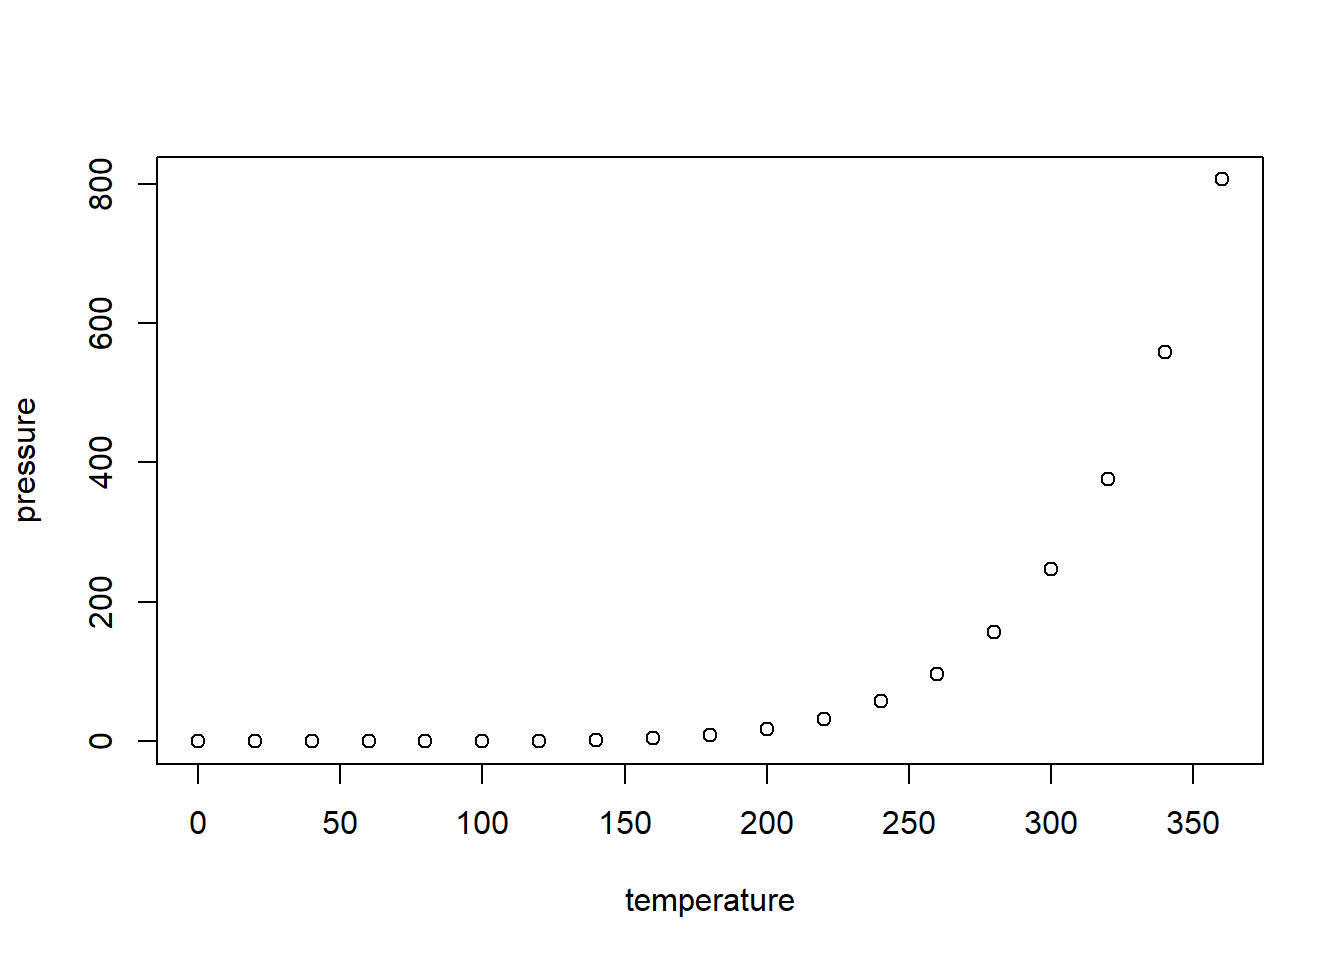
\includegraphics{00-Caderno_Markdown_notes_files/figure-latex/pressure-1.pdf}

Note that the \texttt{echo\ =\ FALSE} parameter was added to the code
chunk to prevent printing of the R code that generated the plot.

\subsection{Math}\label{math}

\[x = y \] \[ x \sim y\] \[ x \apeq y\] \[
   x \approx y
\]

\[   
   p \thickapprox q
\]

\[x < y \]

\[x > y \] \[x \le y \]

\[x \ge y \]

\[x^{n}\]

\[x_{n}\] \[\overline{x}\] \[\hat{x}\]

\[\tilde{x}\]

\[\frac{a}{b}\] \[\sqrt{b^2 - 4ac}\]

\[\frac{\partial f}{\partial x}\]

\[\displaystyle \frac{\partial f}{\partial x}\]

\[\binom{n}{k}\]

\[x_{1} + x_{2} + \cdots + x_{n}\]

\[x_{1}, x_{2}, \dots, x_{n}\] \[\neq \]

\[x \in A\] \[|A|\]

\[x \in A\]

\[x \subset B\]

\[x \subseteq B\]

\[A \cup B\]

\[A \cap B\]

\[X \sim {\sf Binom}(n, \pi)\] (sf for ``slide font'')

\[\mathrm{P}(X \le x) = {\tt pbinom}(x, n, \pi)\] (tt for ``typewriter
type'')

\[P(A \mid B)\]

\[\mathrm{P}(A \mid B)\] (mathrm for ``math roman font'')

\[\{1, 2, 3\}\]

\[\sin(x)\]

\[\log(x)\]

\[\int_{a}^{b}\]

\[\left(\int_{a}^{b} f(x) \; dx\right)\]

\[\left[\int_{-\infty}^{\infty} f(x) \; dx\right]\]

\[\left. F(x) \right|_{a}^{b}\]

\[\sum_{x = a}^{b} f(x)\]

\[\prod_{x = a}^{b} f(x)\]

\[\lim_{x \to \infty} f(x)\]

\[\displaystyle \lim_{x \to \infty} f(x)\]

\subsubsection{Letras Gregas}\label{letras-gregas}

\[\alpha A\]

\[\nu N\]

\[\beta B\] \[\xi\Xi\] \[\gamma \Gamma\]

\[o O\] (omicron)

\[\delta \Delta\] \[\pi \Pi\] \[\epsilon \varepsilon E\]

\[\rho\varrho P\] \[\zeta \sigma \,\!\] \[\sigma \Sigma\]

\[\eta H\] \[\tau T\]

\[\theta \vartheta \Theta\] \[\upsilon \Upsilon\]

\[\iota I\]

\[\phi \varphi \Phi\]

\[\kappa K\]

\[\chi X\]

\[\lambda \Lambda\]

\[\psi \Psi\]

\[\mu M\]

\[\omega \Omega\]

\begin{align*}
a & = b \\
X &\sim {\sf Norm}(10, 3) \\
5 & \le 10
\end{align*}

\[\sum_{n=1}^{10} n^2\]

\[\sum_{n=1}^{10} n^2\]

× \[\times\] -- cross product or cartesian product. ∗ \[*\] --
convolution. ⋅ \[\cdot\] -- dot product ∙ \[\bullet\] -- dot product ⊗
\[\otimes\] -- tensor product. ∘ \[\circ\] -- function composition. Not
a problem for vectors, but can be ambiguous for matrices.

\[\odot\] -- to me the dot makes it look naturally like a multiply
operation (unlike other suggestions I've seen like ⋄) so is relatively
easy to visually parse, but does not have an overloaded meaning as far
as I know.

\subsubsection{Vetores e Matrizes}\label{vetores-e-matrizes}

\[\begin{array}{ccc}
x_{11} & x_{12} & x_{13}\\
x_{21} & x_{22} & x_{23}
\end{array}\]

\[X = \begin{bmatrix}1 & x_{1}\\
1 & x_{2}\\
1 & x_{3}
\end{bmatrix}\]

\[\Theta = \begin{pmatrix}\alpha & \beta\\
\gamma & \delta
\end{pmatrix}\]

\[\begin{vmatrix}a & b\\
c & d
\end{vmatrix}=ad-bc\]

\section{Graficos}\label{graficos}

\subsection{Gerando numeros}\label{gerando-numeros}

\begin{Shaded}
\begin{Highlighting}[]
\FunctionTok{set.seed}\NormalTok{(}\DecValTok{123}\NormalTok{)}
\NormalTok{y }\OtherTok{\textless{}{-}} \FunctionTok{rpois}\NormalTok{(}\DecValTok{1000}\NormalTok{, }\AttributeTok{lambda =} \DecValTok{3}\NormalTok{)}
\FunctionTok{head}\NormalTok{(y)}
\end{Highlighting}
\end{Shaded}

\begin{verbatim}
## [1] 2 4 2 5 6 0
\end{verbatim}

\begin{Shaded}
\begin{Highlighting}[]
\DocumentationTok{\#\# gerou 1000 obs de uma poison}
\end{Highlighting}
\end{Shaded}

\begin{Shaded}
\begin{Highlighting}[]
\FunctionTok{plot}\NormalTok{(y) }\CommentTok{\#grafico basico do R}
\end{Highlighting}
\end{Shaded}

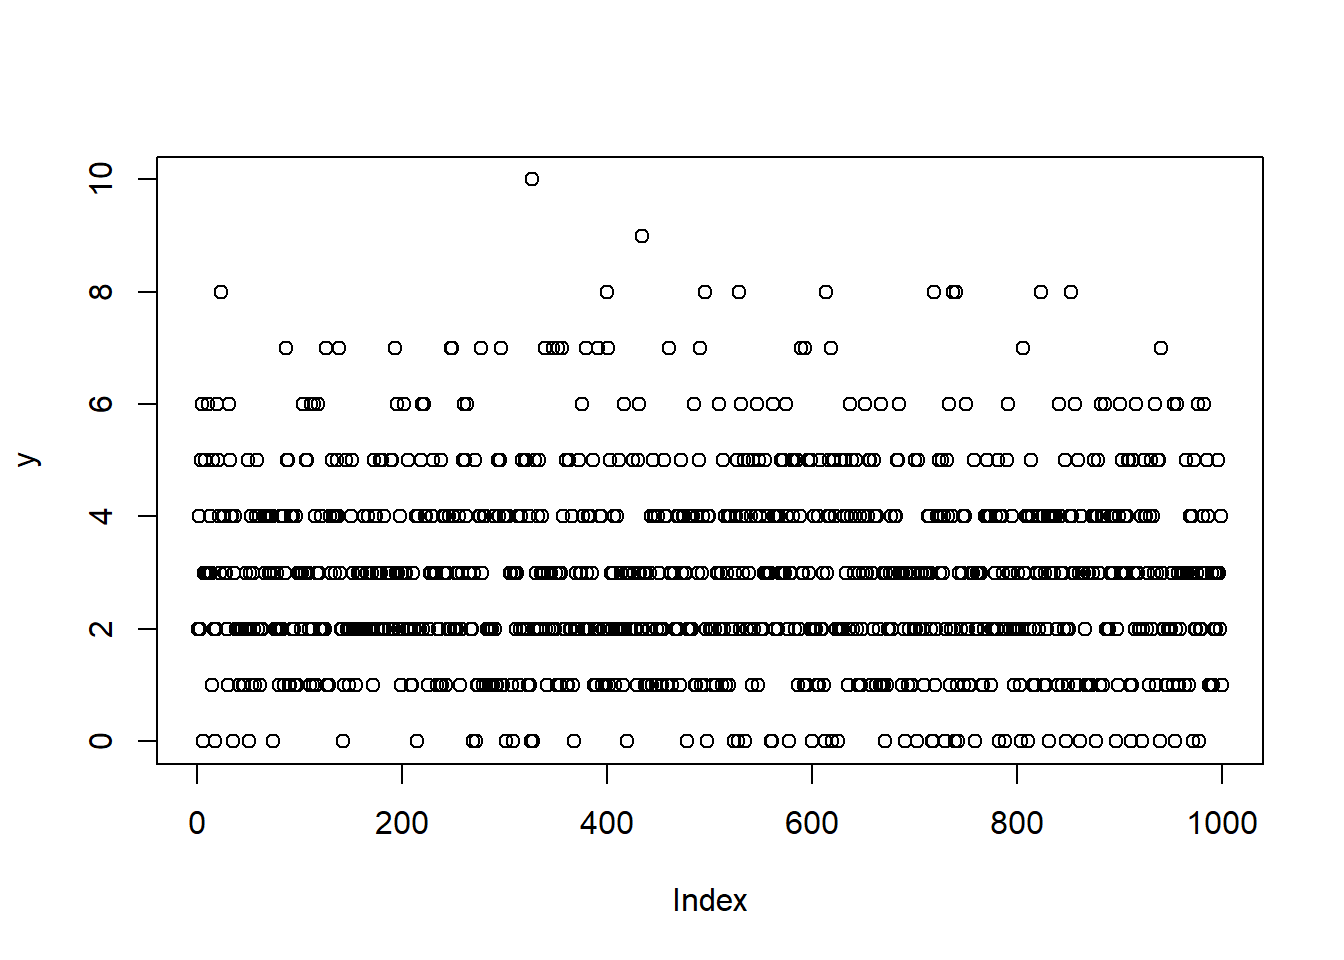
\includegraphics{00-Caderno_Markdown_notes_files/figure-latex/unnamed-chunk-2-1.pdf}

\begin{Shaded}
\begin{Highlighting}[]
\CommentTok{\#ggplot(y, aes(x)) + }
\CommentTok{\#  geom\_histogram( stat = "count")}
\DocumentationTok{\#\# NÃO FUNCIONA PQ PRECISA SER DATA FRAME}
\end{Highlighting}
\end{Shaded}

\subsubsection{Pokemon - Kaggle}\label{pokemon---kaggle}

\begin{Shaded}
\begin{Highlighting}[]
\NormalTok{dados\_pkm }\OtherTok{\textless{}{-}} \FunctionTok{read.csv2}\NormalTok{(}\StringTok{"Pokemon.csv"}\NormalTok{, }\AttributeTok{sep =} \StringTok{","}\NormalTok{)}

\FunctionTok{head}\NormalTok{(dados\_pkm,}\AttributeTok{n =}\DecValTok{10}\NormalTok{)}
\end{Highlighting}
\end{Shaded}

\begin{verbatim}
##    number                name type1  type2 total hp attack defense sp_attack
## 1       1           Bulbasaur Grass Poison   318 45     49      49        65
## 2       2             Ivysaur Grass Poison   405 60     62      63        80
## 3       3            Venusaur Grass Poison   525 80     82      83       100
## 4       3       Mega Venusaur Grass Poison   625 80    100     123       122
## 5       3 Gigantamax Venusaur Grass Poison   525 80     82      83       100
## 6       4          Charmander  Fire          309 39     52      43        60
## 7       5          Charmeleon  Fire          405 58     64      58        80
## 8       6           Charizard  Fire Flying   534 78     84      78       109
## 9       6    Mega Charizard X  Fire Dragon   634 78    130     111       130
## 10      6    Mega Charizard Y  Fire Flying   634 78    104      78       159
##    sp_defense speed generation legendary
## 1          65    45          1     FALSE
## 2          80    60          1     FALSE
## 3         100    80          1     FALSE
## 4         120    80          1     FALSE
## 5         100    80          1     FALSE
## 6          50    65          1     FALSE
## 7          65    80          1     FALSE
## 8          85   100          1     FALSE
## 9          85   100          1     FALSE
## 10        115   100          1     FALSE
\end{verbatim}

\begin{Shaded}
\begin{Highlighting}[]
\FunctionTok{ggplot}\NormalTok{(dados\_pkm, }\FunctionTok{aes}\NormalTok{(type1)) }\SpecialCharTok{+} 
  \FunctionTok{geom\_histogram}\NormalTok{( }\AttributeTok{stat =} \StringTok{"count"}\NormalTok{)}
\end{Highlighting}
\end{Shaded}

\begin{verbatim}
## Warning in geom_histogram(stat = "count"): Ignoring unknown parameters:
## `binwidth`, `bins`, and `pad`
\end{verbatim}

\includegraphics{00-Caderno_Markdown_notes_files/figure-latex/chunk-1-1.pdf}

\subsection{Graficos mais avançados}\label{graficos-mais-avanuxe7ados}

\begin{Shaded}
\begin{Highlighting}[]
\FunctionTok{set.seed}\NormalTok{(}\DecValTok{42}\NormalTok{)}
\NormalTok{df }\OtherTok{\textless{}{-}} \FunctionTok{data.frame}\NormalTok{(}
  \AttributeTok{x =} \FunctionTok{c}\NormalTok{(}\FunctionTok{rpois}\NormalTok{(}\DecValTok{50}\NormalTok{, }\DecValTok{5}\NormalTok{), }\FunctionTok{rpois}\NormalTok{(}\DecValTok{50}\NormalTok{, }\DecValTok{10}\NormalTok{)),}
  \AttributeTok{group =} \FunctionTok{rep}\NormalTok{(}\FunctionTok{c}\NormalTok{(}\StringTok{"A"}\NormalTok{, }\StringTok{"B"}\NormalTok{), }\AttributeTok{each =} \DecValTok{50}\NormalTok{)}
\NormalTok{)}

\FunctionTok{ggplot}\NormalTok{(df, }\FunctionTok{aes}\NormalTok{(x)) }\SpecialCharTok{+}
  \FunctionTok{geom\_bar}\NormalTok{(}\FunctionTok{aes}\NormalTok{(}\AttributeTok{fill =}\NormalTok{ group, }\AttributeTok{y =} \FunctionTok{after\_stat}\NormalTok{(prop)),}
           \AttributeTok{alpha =} \FloatTok{0.5}\NormalTok{, }\AttributeTok{width =} \DecValTok{1}\NormalTok{, }\AttributeTok{position =} \StringTok{"identity"}\NormalTok{) }\SpecialCharTok{+}
  \FunctionTok{stat\_theodensity}\NormalTok{(}\FunctionTok{aes}\NormalTok{(}\AttributeTok{colour =}\NormalTok{ group), }\AttributeTok{distri =} \StringTok{"pois"}\NormalTok{)}
\end{Highlighting}
\end{Shaded}

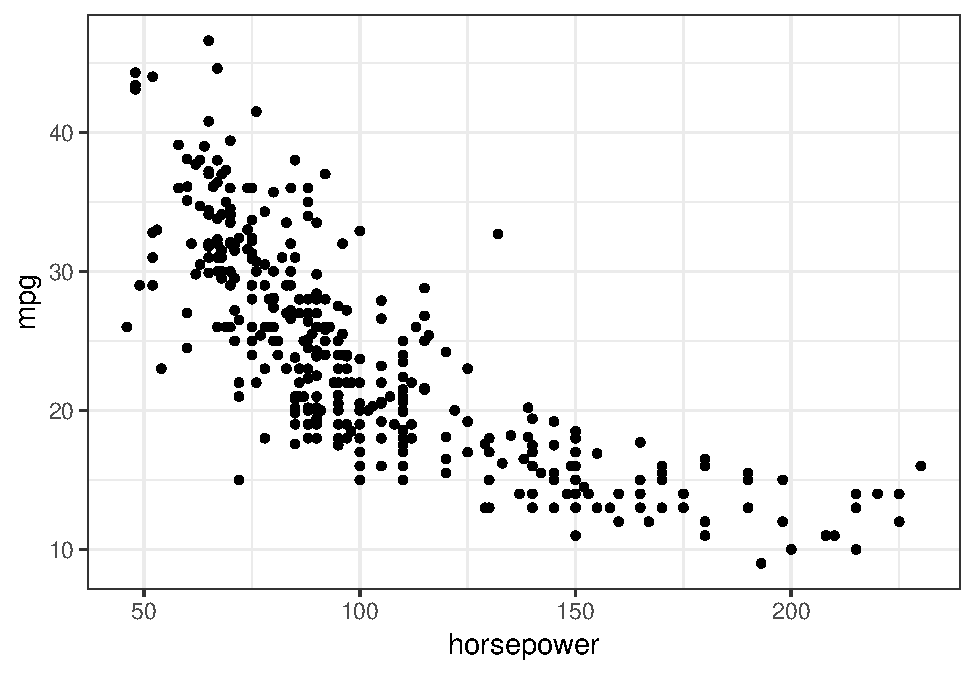
\includegraphics{00-Caderno_Markdown_notes_files/figure-latex/unnamed-chunk-4-1.pdf}

\end{document}
